\section{Parcelando el \'Area de Broca}

\subsection{Distancia coseno con centroide}

Las siguientes Figuras muestran los resultados obtenidos al parcelar el \'Area
de Broca utilizando el m\'etodo de Moreno-Dominguez.

\begin{figure}[h!]
                                                                                                                        
\begin{minipage}[b]{\textwidth}
    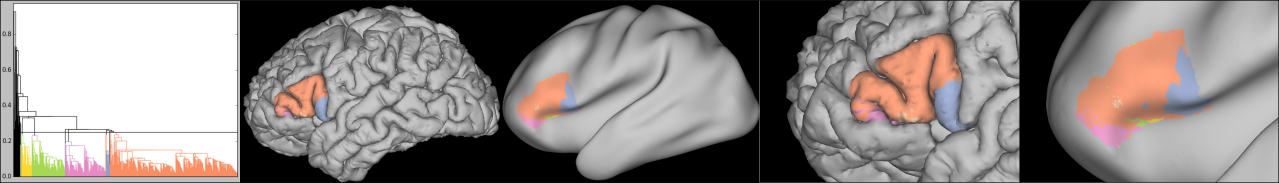
\includegraphics[width=\textwidth]{img/broca/moreno_0.png}
    \caption{M\'etodo Moreno sin preprocesamiento}

\end{minipage} ~
                                                                                                                       
\begin{minipage}[b]{\textwidth}
    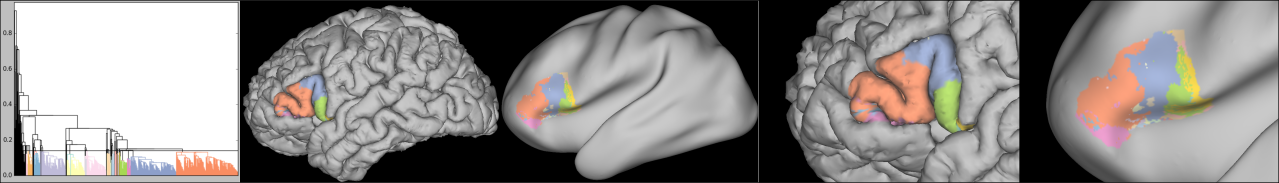
\includegraphics[width=\textwidth]{img/broca/moreno_0_deep.png}
    \caption{M\'etodo Moreno sin preprocesamiento, mayor profundidad en el 
            dendrograma}

\end{minipage} ~

\begin{minipage}[b]{\textwidth}
    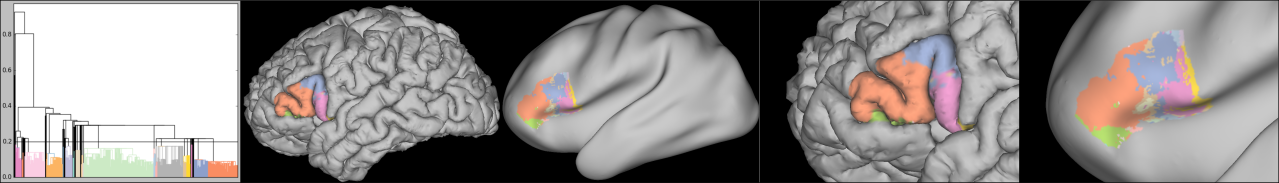
\includegraphics[width=\textwidth]{img/broca/moreno_400.png}
    \caption{M\'etodo Moreno, cuatrocientos pasos de preprocesamiento}

\end{minipage} ~

\begin{minipage}[b]{\textwidth}
    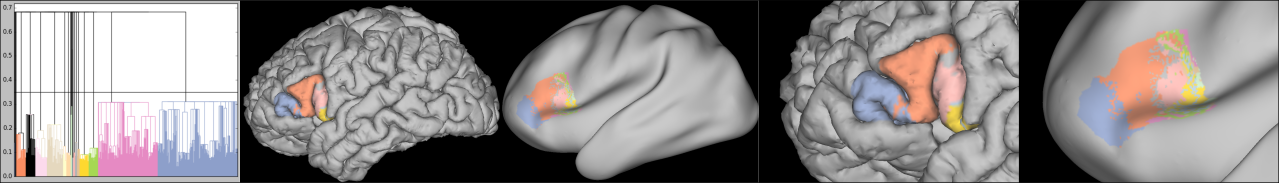
\includegraphics[width=\textwidth]{img/broca/moreno_750.png}
    \caption{M\'etodo Moreno, setecientos pasos de preprocesamiento}

\end{minipage} ~

\end{figure} 


\subsection{Utilizando LogOdds}

Las siguientes Figuras muestran los resultados obtenidos al parcelar el \'Area
de Broca utilizando el m\'etodo de Moreno-Dominguez. El threshold utilizado fue
de $0.25$. \textbf{Los resultados obtenidos luego de normalizar los vectores 
fueron tan malos que no vale la pena incluirlos}.

\begin{figure}[h!]
                                                                                                                        
\begin{minipage}[b]{\textwidth}
    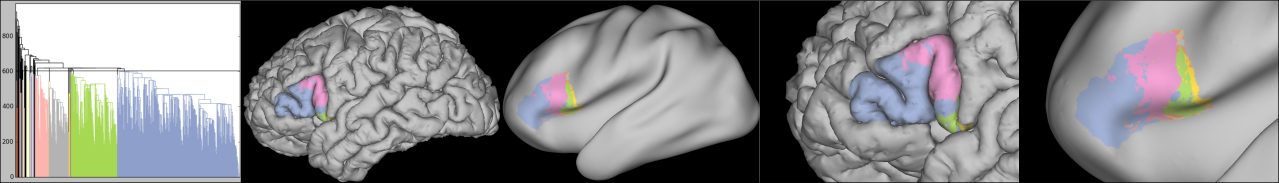
\includegraphics[width=\textwidth]{img/broca/logit_0.png}
    \caption{M\'etodo Logit sin preprocesamiento}
    \label{fig:dmri}
\end{minipage} ~
                                                                                                                        
\begin{minipage}[b]{\textwidth}
    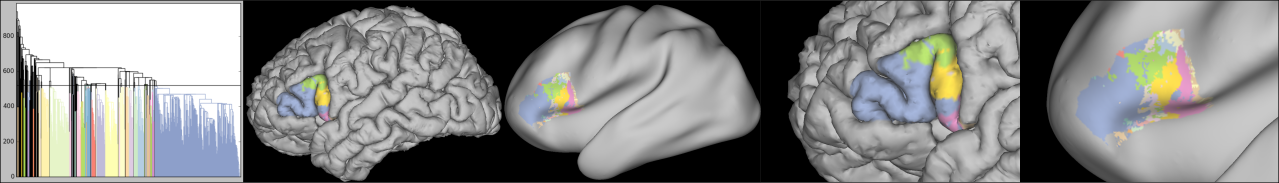
\includegraphics[width=\textwidth]{img/broca/logit_0_deep.png}
    \caption{M\'etodo Logit sin preprocesamiento, mayor profundidad en el 
            dendrograma}

\end{minipage} ~

\begin{minipage}[b]{\textwidth}
    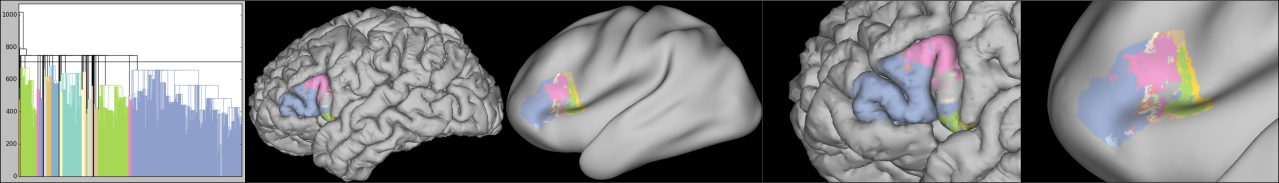
\includegraphics[width=\textwidth]{img/broca/logit_400.png}
    \caption{M\'etodo Logit, cuatrocientos pasos de preprocesamiento}

\end{minipage} ~

\begin{minipage}[b]{\textwidth}
    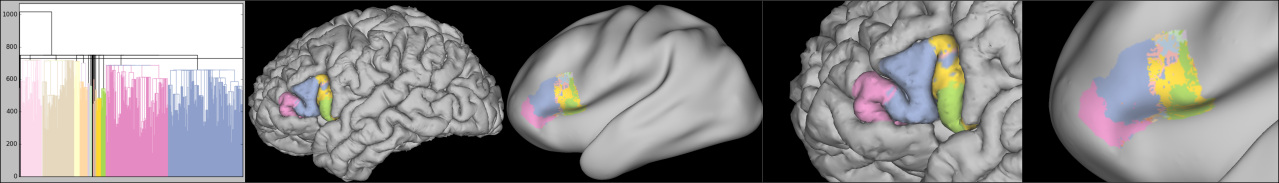
\includegraphics[width=\textwidth]{img/broca/logit_750.png}
    \caption{M\'etodo Logit, setecientos pasos de preprocesamiento}

\end{minipage} ~

\end{figure}


\subsection{Lado a lado}

\begin{figure}[h!]
                                                                                                                        
\begin{minipage}[b]{\textwidth}
    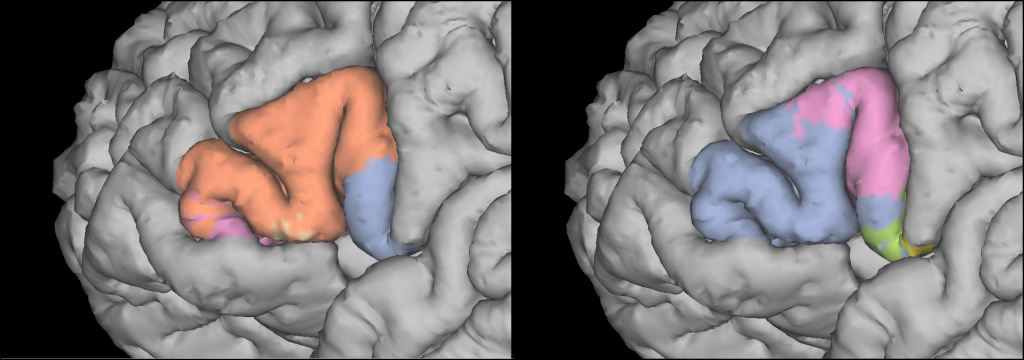
\includegraphics[width=\textwidth]{img/broca/vs_0.png}
    \caption{M\'etodo Moreno (izquierda) y Logit (derecha) sin preprocesamiento}
\end{minipage} ~

\end{figure}

\begin{figure}[h!]                  
                                                                                                                        
\begin{minipage}[b]{\textwidth}
    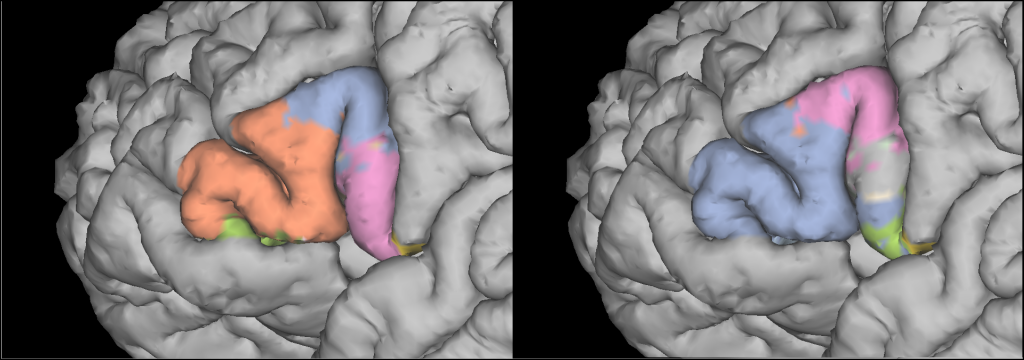
\includegraphics[width=\textwidth]{img/broca/vs_400.png}
    \caption{M\'etodo Moreno (izquierda) y Logit (derecha). Cuatrocientos pasos de preprocesamiento}
\end{minipage} ~

\end{figure}

\begin{figure}[h!]

\begin{minipage}[b]{\textwidth}
    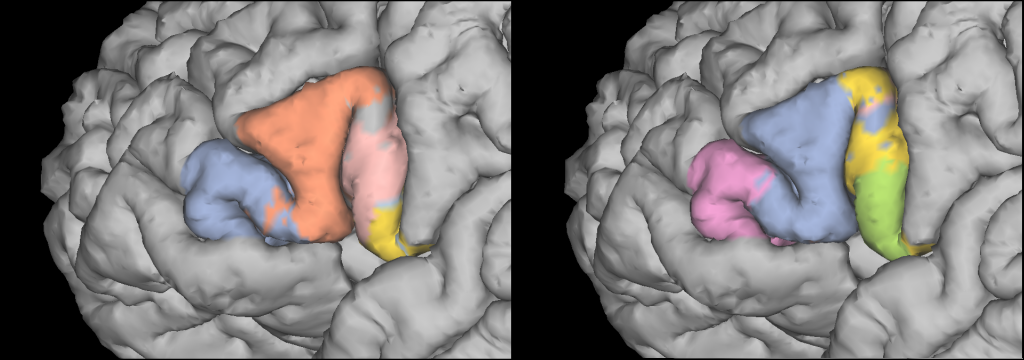
\includegraphics[width=\textwidth]{img/broca/vs_700.png}
    \caption{M\'etodo Moreno (izquierda) y Logit (derecha). Setecientos pasos de preprocesamiento}

\end{minipage} ~

\end{figure}
 
